\chapter{NOTICIAS PODCAST}

\section{\textquestiondown Que son los feed de noticias?}

El feed \footnote{Suministrar informaci\'{o}n} pueden ser m\'{a}s que t\'{i}tulos y enlaces, esto permite a los usuarios 
obtengan las \'{u}ltimas actualizaciones del sitio a diferentes dispositivos enviados desde un sitio web.

Los feeds pueden ser cualquier cosa de pocos titulares y enlaces a historia a todo el contenido del sitio, despojados
de su trazado y con metadatos aplicados generosamente. Sindicaci\'{o}n de contenidos permite a los usuarios experimentar
un sitio en varios dispositivos y ser\'{a}n notificados de cambios a trav\'{e}s de una variable de servicios. Puede 
variar desde una simple lista de enlaces enviados desde un sitio a otro a los inicios de la Web Sem\'{a}ntica.\cite{hammersley2005developing}

RSS y Atom son XML formatos para mensajes y otra informaci\'{o}n que es actualizada frecuentemente.
Los documentos que son escritos en estos formatos son llamados newfeeds or feed.\cite{wittenbrink2005rss}

Se define RSS \footnote{Really Simple Syndication} como un formato basado en XML \footnote{Extensible Markup Language: designado para almacenar y transportar datos} para compartir contenido del sitio web.

Si un sitio web quiere compartir y publicar parte de su contenido a otros sitios en el mismo tiempo, el editor puede crear un
documento RSS. Este documento se puede publicar en el sitio web y cualquier usuario puede leer y utlizar diferentes sitios al mismo
tiempo. \cite{zeki2004rss}

Se utiliza la tecnolog\'{i}a feed de noticias para tener al usuario a los \'{u}ltimos contenidos en la aplicaci\'{o}n web
y este pueda notificarle via correo electronico del mismo con el t\'{i}tulo, descripci\'{o}n y categor\'{i}a al que pertenece.

\section{Sintaxis: RSS como XML formato}

Para muchos desarrolladores \textquotedblleft XML\textquotedblright y \textquotedblleft RSS\textquotedblright son sinominos. Se utiliza ambas tecnolog\'{i}as para el intercambios de informaci\'{o}n
en la Web.

Muchos sitios web identifican sus fuentes de noticias a trav\'{e}s de un bot\'{o}n de color naranja marcado \textquotedblleft XML\textquotedblright. Para muchos usuarios, y tambi\'{e}n para muchos desarrolladores \textquotedblleft XML\textquotedblright  y \textquotedblleft RSS\textquotedblright son sin\'{o}nimos. De hecho, todas las versiones del formato RSS y Atom son XML aplicaciones. Desde XML en s\'{i} es un metalenguage para definir idiomas par el intercambio de informaci\'{o}n en la
Web, los formatos de fuentes son tambi\'{e}n a menudo se llama \textquotedblleft dialectos XML\textquotedblright  o \textquotedblleft XML vocabularios \textquotedblright. A la fecha, RSS es el vocabulario, 
excepto XML de mayor \'{e}xito para tal XHTML, la versi\'{o}n XML de HTML.\cite{wittenbrink2005rss}

Se identifica un icono de color naranja que contiene en su interior un circulo y dos lineas curvas de color blanco para conocer
que la aplcaci\'{o}n web cuenta con subscripci\'{o}n.

\section{RSS 0.90}

Con RSS es posible integrar t\'{i}tulos desde otros sitios en la portada. Los usuarios deberian personalizar y suscribirse 
a un n\'{u}mero de canales que ofrece un canal de noticias RSS.


RSS fue inicialmente una abreviatura de \textquotedblleft RDF Site Summary \textquotedblright (Para obtener informaci\'{o}n acerca de RSS como
\textquotedblleft RDF Site Summary\textquotedblright consulte el Cap\'{i}tulo 3, Para una explicaci\'{o}n detallada del t\'{e}rmino, ver secci\'{o}n
3.1 RDF Fundamentos). Con RSS, es posible integrar los titulares de otros sitios con enlaces a estos sitios en el 
portal. El usuario puede personalizar el portal y suscribirse a un n\'{u}mero de sitios que ofrecen datos RSS.
De esta manera, My Netscape ten\'{i}a a su disposici\'{o}n una gran cantidad de contenidos adicional, que mantiene
a los usuarios en el sitio ya; los proveedores de datos RSS recibida tr\'{a}fico en el objetivo adicional m\'{a}s
importante de muchos sitios web en los tiempos de la boom de las punto-com. Puesta que es f\'{a}cil de convertir 
RSS a HTML. otros sitios pronto empezaron a utilizar la misma tecnolog\'{i}a. Slashdot pronto utiliza RSS en lugar
de su propio formato de t\'{i}tulo, y herramientas fueron desarrolladas para crear y el proceso de RSS en los 
lenguages de programaci\'{o}n comunes.\cite{wittenbrink2005rss}


Se tiene una tecnolog\'{i}a RSS, de tal forma que pueda obtener informaci\'{o}n de otros sitios en beneficio de
tener un lector de acceder a las noticias y no necesariamente acceder al sitio web.

\section{Los elementos de RSS 0.91}

Un importante version de Netscape RSS 0.91 a comparaci\'{o}n de RSS 0.90 de validar documentos de este formato
a comparacion de un DTD \footnote{Es un tipo de documento: define la estructura y legal elementos y atributos de un documento
XML}. 

La definitiva fuente de informaci\'{o}n respecto RSS 0.91 es la especificación de esta misma, pero para su 
conveniencias nosotros tenemos un diagrama Fig 2.1. Cada caja en el diagrama representa un elemento XML, 
y una fila indica contenci\'{o}n.\cite{johnson2006rss}

\begin{center}
	Elementos que componen un canal de noticias RSS 0.91.
\end{center}

\begin{minipage}{1.0\textwidth}
	\centering
	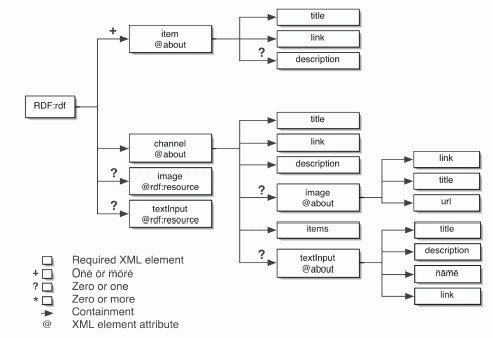
\includegraphics[scale=0.8]{rss091}
	\captionof{figure}{los elementos XML que componen RSS 0.91}
	\source{fuente: \cite{johnson2006rss}}

\end{minipage}


\section{RSS 1.0}

Un importante desarrollador Rael Dornfest quiso expandir el alcande de RSS. Por lo tanto ellos introducen
RDF \footnote{Resource Description Framework Schema: un set de clases con ciertas propiedades.} y tambi\'{e}n un nuevo mecanismo, espacio de trabajo XML.

Otros desarrolladores importantes, sin embargo, entre ellos Rael Dornfest, que trabajaba como director de
tecnolog\'{i}a de O'Reilly, quer\'{i}a ampliar el alcance de RSS utilizando para otro prop\'{o}sitos y lo
conectan con formatos adicionales. Por lo tanto, se reintrodujeron RDF y tambi\'{e}n introdujo un nuevo
mecanismo, el espacio de nombres XML. Una especificaci\'{o}n relacionado fue publicado en diciembre de 2002;
los desarrolladores llaman el formato que se describe, RSS 1.0.\cite{johnson2006rss}

Esta norma, lanzado en diciembre de 2000, trajo dos cambios importantes en el mundo RSS: la introducci\'{o}n
de RDF y con ella una introducci\'{o}n de espacios de nombres.\cite{hammersley2005developing}
 
\subsection{Los elementos de RSS 1.0}

Comparando los RSS 0.91 y RSS 1.0 diagramas, tu puedes ver los formatos son significativos diferentes.
Aqui son las palabras diferentes:

\begin{itemize}

\item Un típico flujo RS 1.0 es más largo y más complejo, pero no lo hace incluir tantos metadatos como el
equivalente RSS 0.91 newfeed.

\item RSS 1.0 es más complejo, pero sólo porque es más flexible y extensible.

\item El elemento raíz es <RDF:rdf> en lugar de <rss>.

\item Las noticias existen como hijos de elemento raíz del documento y no como hijos del elemento <channel>,
como lo hacen en RSS 0.91.

\item Las noticias deben ser declaradas dentro del <channel> como recursos DRF. \par

\begin{center}

Elementos que componen un canal de noticias RSS 1.0

\end{center}

\begin{minipage}{1.0\linewidth}
	\centering
	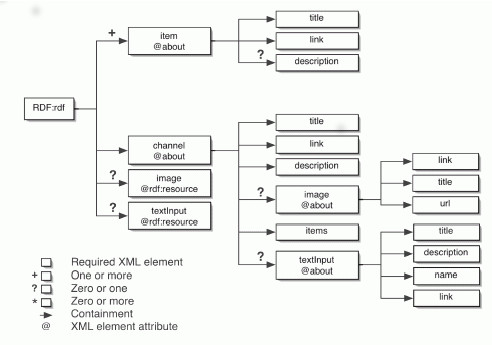
\includegraphics[scale=0.8]{rss010}
		\captionof{figure}{Los elementos XML que componen RSS 1.0}
		\source{fuente: \cite{johnson2006rss}}
\end{minipage}

\item <image> y <textinput> elementos deberian ser declarado dentro los <RDF:rdf> elementos son RDF
si han de ser incluidos dentro de la <channel> elemento.

\item Muchos elementos de metadatos, tales como  <pubDate>, <lastBuild-Time>, <skipDays>,
<skipHours>, <managingEditor>, y <webMaster> faltan del para. Estos se pueden añadir según sea necesario
mediante el uso de RSS 1.0 módulos, que se describen en la siguiente sección.\cite{johnson2006rss}

\end{itemize}

\section{RSS 2.0}

Se tiene RSS 2.0 esencialmente define sintaxis, El soporte de RSS 2.0 es considerado de baja especificaci\'{o}n
ya que es uno de los formatos de mayores ventajas.

Hoy en d\'{i}a, es el formato RSS feed m\'{a}s utilizado. Es caracter\'{i}stico de este formato no especifique,
o para dejar a los desarrolladores de aplicaciones para especificar: las conexiones entre Datos RSS, por una 
parte, entre otros formatos de contenido, datos/formatos de metadatos, y entornos de publicaci\'{o}n.\cite{wittenbrink2005rss}

\subsection{Los elementos de RSS 2.0}

\'{U}ltimamente RSS es ampliamente el formato m\'{a} usado. las conexiones entre RSS datos, contenidos de datos
en formatos/metadatos en otros entornos.

Hoy en d\'{i}a, es el formato RSS m\'{a}s utilizado. Es caracter\'{i}stico de este formato no especifique,
o para dejar a los desarrolladores de aplicaciones para especificar: las conexiones entre Datos RSS, por una
parte, entre otros formatos de contenido, datos/formatos de metadatos, y entornos de publicaci\'{o}n, por otro
lado. Esencialmente, RSS 2.0 define la sintaxis, en tanto que significado y el uso de determinaron mediante el
uso de ejemplos. Los partidiarios de RSS 2.0 consideran este bajo nivel de especificaci\'{o}n de una de las
mayores ventajas del formato, mientras que los partidiarios de las versiones de RSS alternas ven como su mejor
momento de debilidad.\cite{wittenbrink2005rss}

Esto, en realidad es la clave para el \'{e}xito de la RSS 2.0. La cosa m\'{a}s simple hay que hacer para hacer la validaci\'{o}n
de alimentaci\'{o}n es muy sencillo de hecho (vease el ejemplo 4.2). Si bien esto no es ninguna ayuda cuando usted est\'{a}
tratando de transmitir informaci\'{o}n compleja, como con RSS 1.0 o si usted est\'{a} tratando de construir un sistema centrada
en el documento completo, al igual que con Atom, es muy \'{u}til para muchas otras aplicacion.\cite{hammersley2005developing}

Los RSS 2.0 especificación provee una detallada descripci\'{o}n de cada elemento permitido en un RSS 2.0
newfeed. Tu puedes encontrar la especificaci\'{o}n aqu\'{i}  http://blogs.law.harvard.edu/tech/rss. Resumiendo
el XML que componen RSS 2.0, usando la misma notaci\'{o}n como nuestra previa figura, con un toque.\cite{johnson2006rss}

Se tiene un nueva version la cual conlleva las ventajas de las anteriores versiones y esta pueda ser manipulable por
lectores en equipos como agregadores online, tambien implementadas en applicaciones web.

\begin{center}
	Elementos que componen un canal de noticias RSS 2.0
\end{center}

\begin{minipage}{1.0\linewidth}
	\centering
	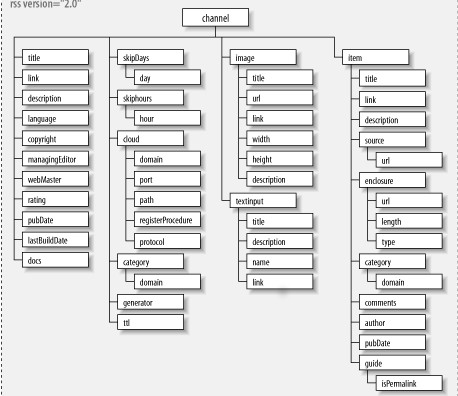
\includegraphics[scale=0.8]{rss020}
		\captionof{figure}{Los elementos XML que componen RSS 2.0}
		\source{fuente: \cite{johnson2006rss}}
\end{minipage}

\subsection{Plataforma Educativa LAEL}

Se tiene la realizaci\'{o}n de la subscripci\'{o}n de un canal de noticias, para ello el usuario deber\'{i}a
de encontrarse autentificado. 

\begin{minipage}{1.0\linewidth}
\centering
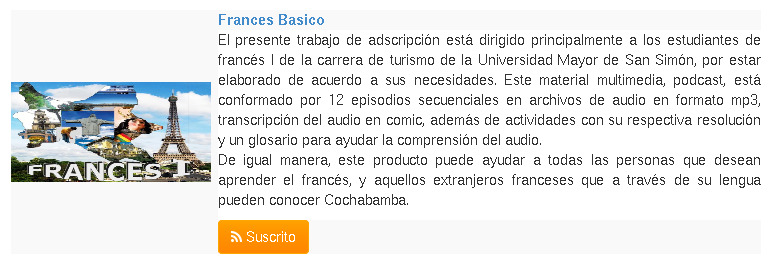
\includegraphics[scale=0.5]{basicFranceSubscribed}
\captionof{figure}{Subscripci\'{o}n Programa Aprendizaje Frances B\'{a}sico}
\source{fuente: (Propia)}
\end{minipage}

Haciendo uso de un navegador como Firefox, se puede utilizar un lector de noticias que encuentra disponible
y poder identifcar los diferentes elementos que contiene un feed de noticas: T\'{i}tulo, Fecha Liberaci\'{o}n
y Descripti\'{o}n.
 
\begin{minipage}{1.0\linewidth}
\centering
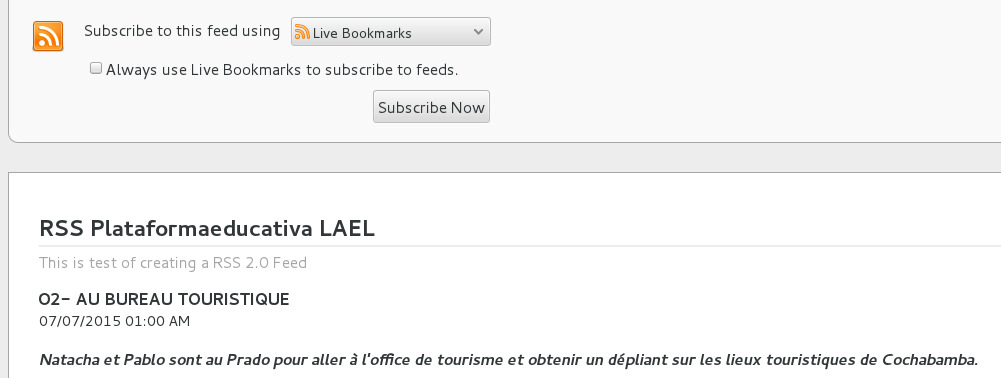
\includegraphics[scale=0.4]{basicFranceRssFirefox}
\captionof{figure}{Episodio1: Elemento canal de noticias}
\source{fuente: (Propia)}
\end{minipage}


\subsection{Las nueve versiones incompatibles de RSS}

Un influente blogger nombre Mark Pilgrim tiene que ser seguidor el desarrollador RSS de cerca, y el tiene que hacer
algunas importantes contribuciones. Trabajando con Sam Ruby, otro influente blogger, Pilgrim desarrollo servicio validacion de noticias lugar http://www.feedvalidator.org/ que maneja toda la comúnmente uso de RSS y Atom noticas
formato. 
Pilgrim señalaron que había nueve incompatibilidades versiones de RSS. Resumiendo estas incompatibles versiones y
autores, fecha y estado de cada una.\cite{johnson2006rss}

\begin{minipage}[b]{\hsize}\centering

\begin{tabular}{>{\centering\arraybackslash}m{.05\linewidth} |>{\centering\arraybackslash}m{.17\linewidth}|>{\centering\arraybackslash}m{.1\linewidth}|>{\centering\arraybackslash}m{.2\linewidth}|>{\centering\arraybackslash}m{.4\linewidth}}

& \textbf{Liberado por} & \textbf{Fecha} & \textbf{Estado} & \textbf{Nota} \\
\hline

\textbf{RSS 0.90} & Libby/Netscape & Enero 1999 & \textbf{Obsoleto} y rara vez se encuentra en la naturaleza & RDF- basado formato. \\
\hline

\textbf{RSS 0.91 } & Libby/Netscape & Julio 1999 & \textbf{Obsoleto} pero ampliamente usado & XML-basado con DTD; caído todos los elementos RDF; Añadido soporte para módulos. \\
\hline 

\textbf{RSS 0.91 (UserLand) } & Winer/Userland & Junio 2000 & \textbf{Obsoleto} pero ampliamente usado & caído DTD. \\
\hline 

\textbf{RSS 1.0} & RSS-DEV & Diciembre 2000 & \textbf{Viable} y ampliamente usado & RDF-basado formato nuevamente.\\
\hline

\textbf{RSS 0.92} & Winner/Userland & Diciembre 2000 & \textbf{Obsoleto} pero ampliamente usado & Contenido tipo de <description> elemento cambiado desde texto plano\\
\hline

\textbf{RSS 0.93} & Winer/Userland & Abril 2001 & \textbf{Obsoleto} y rara vez que se encuentra en la naturaleza & Aniadidp <pubDate> y <expirationDate> elementos. tambien permite multiples <enclousure> elementos por <item> \\
\hline

\textbf{RSS 0.94} & Winer/Userland & Verano 2002 & \textbf{Obsoleto} y rara vez que se encuentra en la naturaleza & eliminado <expirationDate> elemento. Especificación ya no está disponible en línea\\
\hline

\textbf{RSS 2.0} & Winer/Userland & Agosto 2002 & \textbf{Viable} y ampliamente usado. Final version de RSS & Permite adición de nuevos elementos siempre y cuando se definen por Espacio de nombres XML\\
\hline 

\textbf{RSS 2.0.1} & Winer/Harvard & Julio 2003 & Menor cambio a RSS 2.0 & Agregado elemento <rating>\\
\hline 

\end{tabular}

\captionof{table}{Las nueve versiones incompatibles de RSS}
\source{fuente: \cite{johnson2006rss}}
\end{minipage}

\section{El nuevo estandar: Atom}

A principios del 2003 un grupo de blooggers desilucionados con estado de newfeeds publicaron un nuevo estandar API
\footnote{Es un conjunto particular de reglas y especificaci\'{o}n que el programas pueden seguir para comunicarse entre si} el cual deberia ser conocido como Atom.

Atom es un formato de documento basado en XML que describe las listas de informaci\'{o}n relacionada conocida como
\textquotedblleft feeds\textquotedblright. Feeds se componen de una serie de elementos, conocidos como \textquotedblleft 
entradas \textquotedblright, cada uno con un conjunto extensible de metadatos adjunto.%\cite{nottingham2005atom}

Si piensas Atom es una mejora sobre RSS o solamente otro formato, como un aplicación de blog usted 
tendra que aprender Atom. Todo el mayor servidor blog si soporta Atom ahora o tiene planes para hacer, y Blogger.com,
uno de los largos servicios blogging, ofrece solo Atom noticias - no RSS.\cite{johnson2006rss}


\subsection{Los elementos de Atom}


Nosotros tenemos usado la notación <<text>>, <<person>>, y <<fecha>> a indicar cuales elementos son constructores
comunes. Requeridos elementos son compartidos.

Elementos que componen un canal de noticias Atom.

\begin{figure}[!ht]
\centering
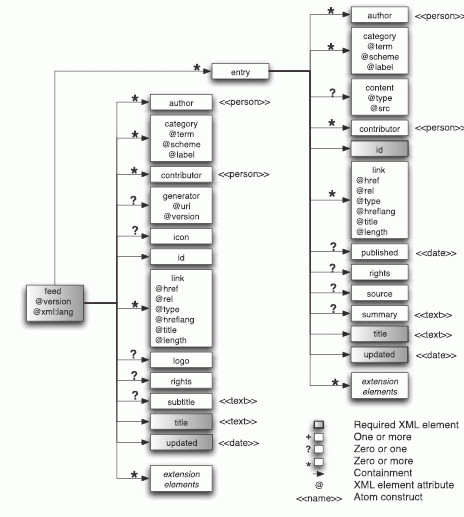
\includegraphics[scale=0.8]{elementsXML}
\caption{Los elementos XML que conforman un servicio de noticias Atom}
\source{fuente: \cite{johnson2006rss}}
\end{figure}


Algunos requisitos importantes no son evidentes a partir de este diagrama formato Atom, Por lo tanto permiteme
revisar ellos. Primero, el nivel feed requisito.

\begin{itemize}

\item El feed debe contener un <id> elemento.
\item El feed debe contener un <link> con rel="self" que contiene un enlace to el feed mismo. Esto hace posible para
un programa, cual puede tener solo una copia de un documento de noticias, a encontrar la URL de las noticias.
\item El feed debe incluir un solo enlace, significando un <link> elemento con rel="alternate" - tipicamente un enlace
alternativo de un alimento hace referencia a una alternativa representación de la alimentación.
\item El autor debe ser especifico lugar el nivel feed o en cada individual entrada.

\end{itemize}

Y ahora, en cada nivel requiere.

\begin{itemize}

\item Cada entrada debe contener un <id> elemento.
\item Si la entrada no tienen un <content> elemento, deberia tener una alternativo enlace. Un enlace alternativo es su enalce
permanente, un enlace permanente entradas representacion web.
\item Un enlace puede tener multiples enlaces alternativos para diferentes lenguajes y tipos de contenidos, pero una entrada
deberia no contener mas que una enlace alternativo para cada combinacion de languages y tipo de contenido.
\item La entrada deberia incluir un <summary> elemento si el contenido es no facilmente leible, por ejemplo es no <content> 
elemento, el <content> elemento contiene algun otro texto, o el <content> referencia de elementos contenido en otros lugares.\cite{johnson2006rss}

\end{itemize}

\subsection{Podcasting con Atom}

La Figura 2.5, muestra la evoluci\'{o}n y los distintos caminos tomados por los formatos 
RSS y Atom.

Podcasting originado como una caracteristica de RSS, pero a medida que el mundo se mueve Atom como el nuevo estándar.
Los podcasters también lo hará - y para buenas razones. Atom puede soportar podcasting a travez del elemento <link>.
Como es el caso con RSS 2.0-basado podcasts, usted puedes tener solo un podcast por entrada. Pero con Atom, tu puedes
tener diferentes representacion por cada lenguage y por cada tipo de contenido.\cite{johnson2006rss}

Cronolog\'{i}a del tiempo respecto Atom.

\begin{figure}[!htb]
\centering
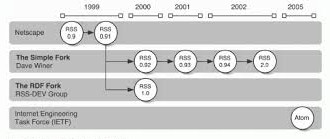
\includegraphics[scale=1]{newsFeed}
\caption{News feed árbol formato}
\source{fuente: \cite{johnson2006rss}}
\end{figure}
